\documentclass[utf8]{beamer}
\mode<presentation>
\usepackage[spanish]{babel}
\usepackage{multicol}
\useoutertheme{infolines} 
\usepackage{graphicx}

\usetheme{Boadilla}
\usecolortheme{crane}
\useoutertheme{shadow}
\useinnertheme{rectangles}

\title[Comic It!]{Comic It!}
\subtitle{Creando historietas}
\author[Ana Arias,Liliana Ramos,Denny Schuldt]
{Ana Arias \newline Liliana Ramos\newline Denny Schuldt}
\institute[ESPOL]
{
  Escuela Superior Politécnica del Litoral

}
\date{\today}

\AtBeginSection{
\begin{frame}
  \frametitle{Índice}
  \tableofcontents[currentsection]   
\end{frame}
}

\AtBeginSubsection{
\begin{frame}
  \frametitle{Índice}
  \tableofcontents[currentsection,currentsubsection]
\end{frame}
}

\begin{document}

\frame{\titlepage}

\begin{frame}
  \frametitle{Índice}
  \tableofcontents
\end{frame}

\section{Comiqueando!}
\subsection{Descripción}

\begin{frame}
  \frametitle{Descripción}

\begin{center}
		\begingroup
			
\includegraphics[width=0.30\textwidth]{imagenes/comicit.jpg}
		\endgroup
	\end{center}

  \begin{block}{Diversión}
Comic It! es una aplicación súper divertida para Tablets con sistema operativo Android. Aquí podrás realizar caricaturas de tu vida diaria o imaginarte alguna y la obtendrás de una manera muy sencilla y llamativa.
  \end{block}
       
 
\end{frame}


\subsection{Componentes}

\begin{frame}
  \frametitle{Iconos}

       
 	\begin{center}
		\begingroup
			
\includegraphics[width=0.30\textwidth]{imagenes/icono1.png}
			\hspace{1mm}
			
\includegraphics[width=0.30\textwidth]{imagenes/icono2.png}
			\hspace{1mm}
			
\includegraphics[width=0.30\textwidth]{imagenes/icono3.png}
			\hspace{1mm}
			
\includegraphics[width=0.30\textwidth]{imagenes/icono4.png}
			\hspace{1mm}
			
\includegraphics[width=0.30\textwidth]{imagenes/icono5.png}
			\hspace{1mm}
			
\includegraphics[width=0.30\textwidth]{imagenes/icono6.png}
			\hspace{1mm}
			
\includegraphics[width=0.30\textwidth]{imagenes/icono7.png}
		\endgroup
	\end{center}


\end{frame}


\subsection{Características implementadas}



\begin{frame}
  \frametitle{Tabs}
 

  	\begin{center}
		\begingroup
			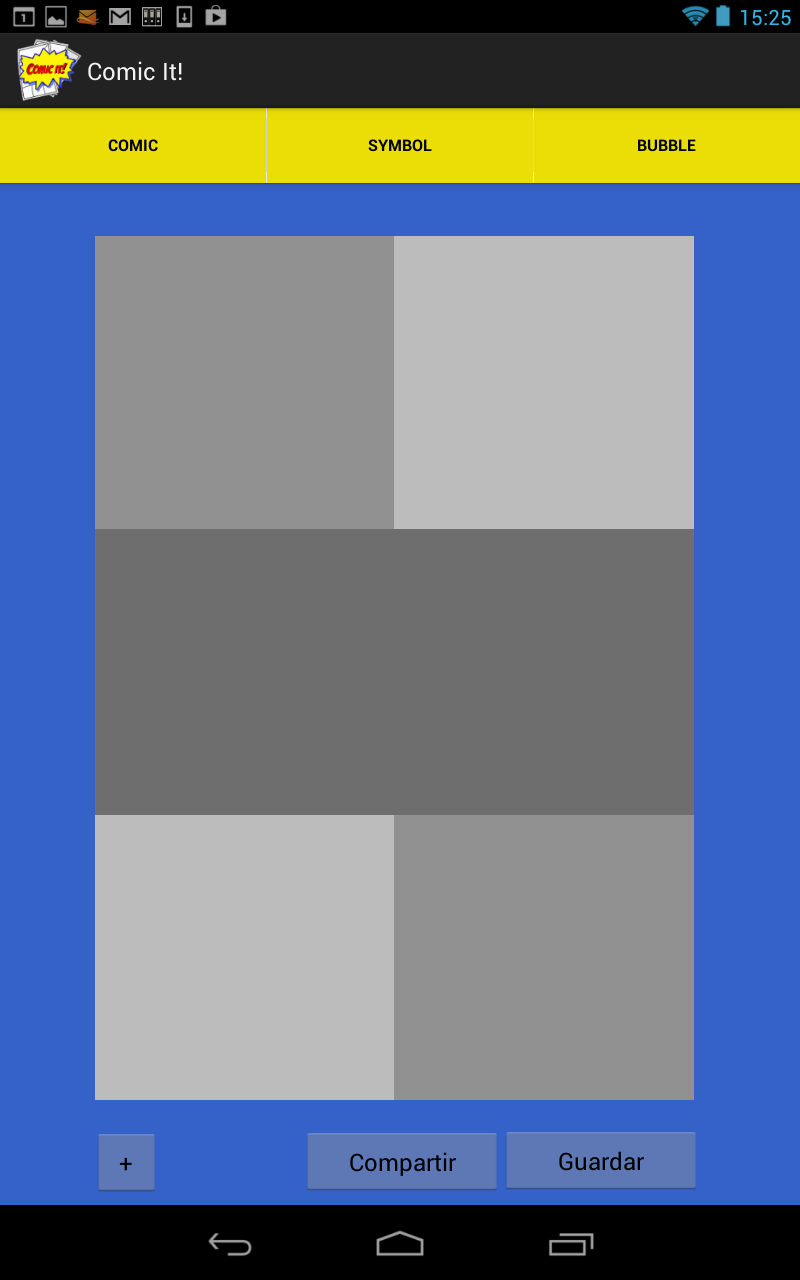
\includegraphics[height=4cm,width=2.8205cm]{imagenes/plantilla.png}
			\hspace{1mm}
			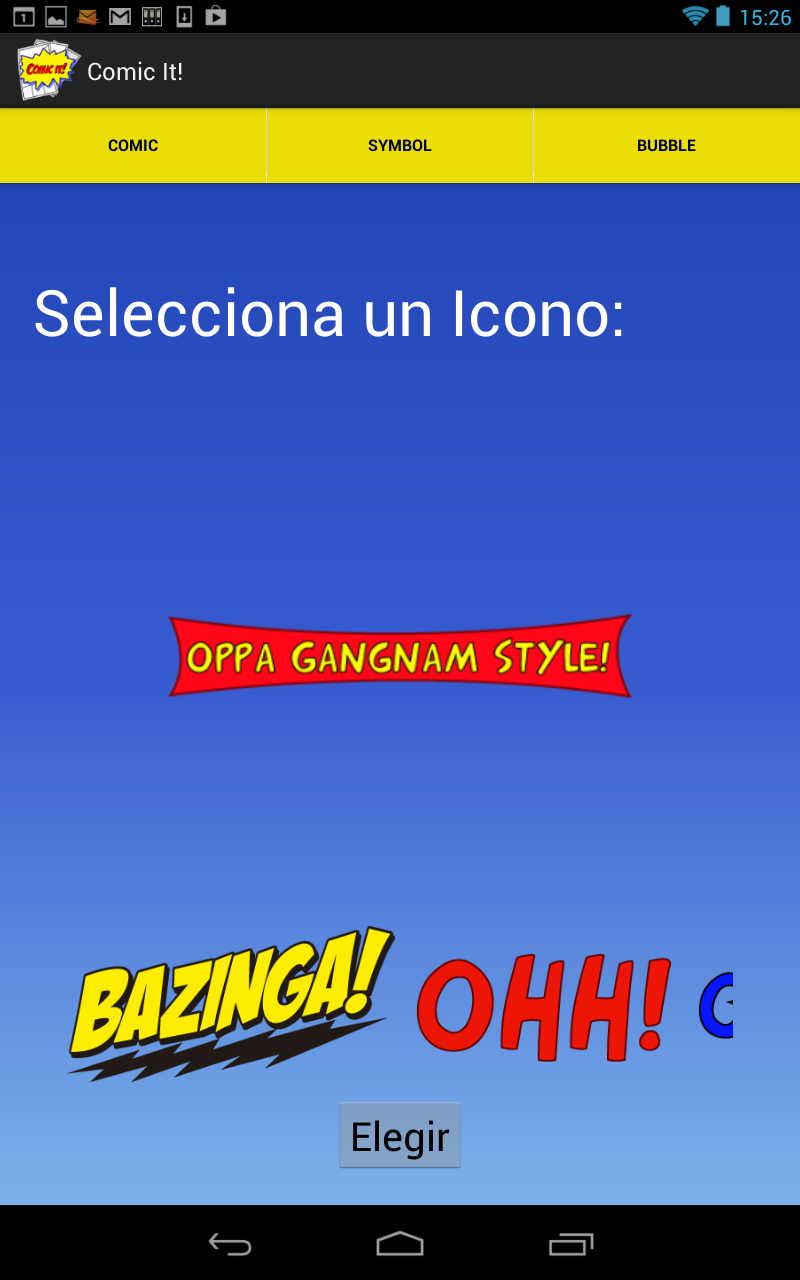
\includegraphics[height=4cm,width=2.8205cm]{imagenes/iconos.png}
			\hspace{1mm}
			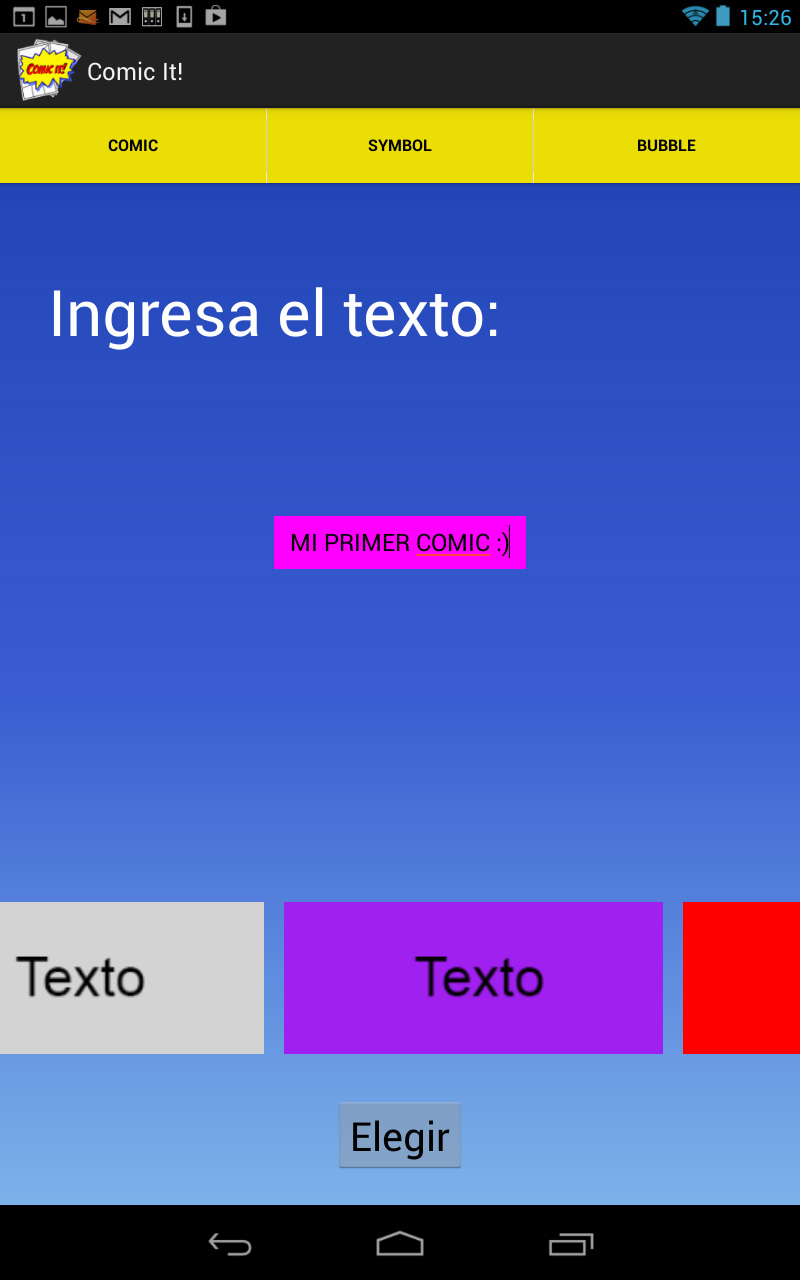
\includegraphics[height=4cm,width=2.8205cm]{imagenes/textos.png}
		\endgroup
	\end{center}

  \begin{block}{}
Comic It! se maneja mediante Tabs las cuales son el Comic, los íconos y los textos que podrás tener. Cada una funciona de manera independiente y son los que le dan el flujo a nuestra aplicación.
  \end{block}

\end{frame}

\begin{frame}
  \frametitle{Cámara}
 

  	\begin{center}
		\begingroup
			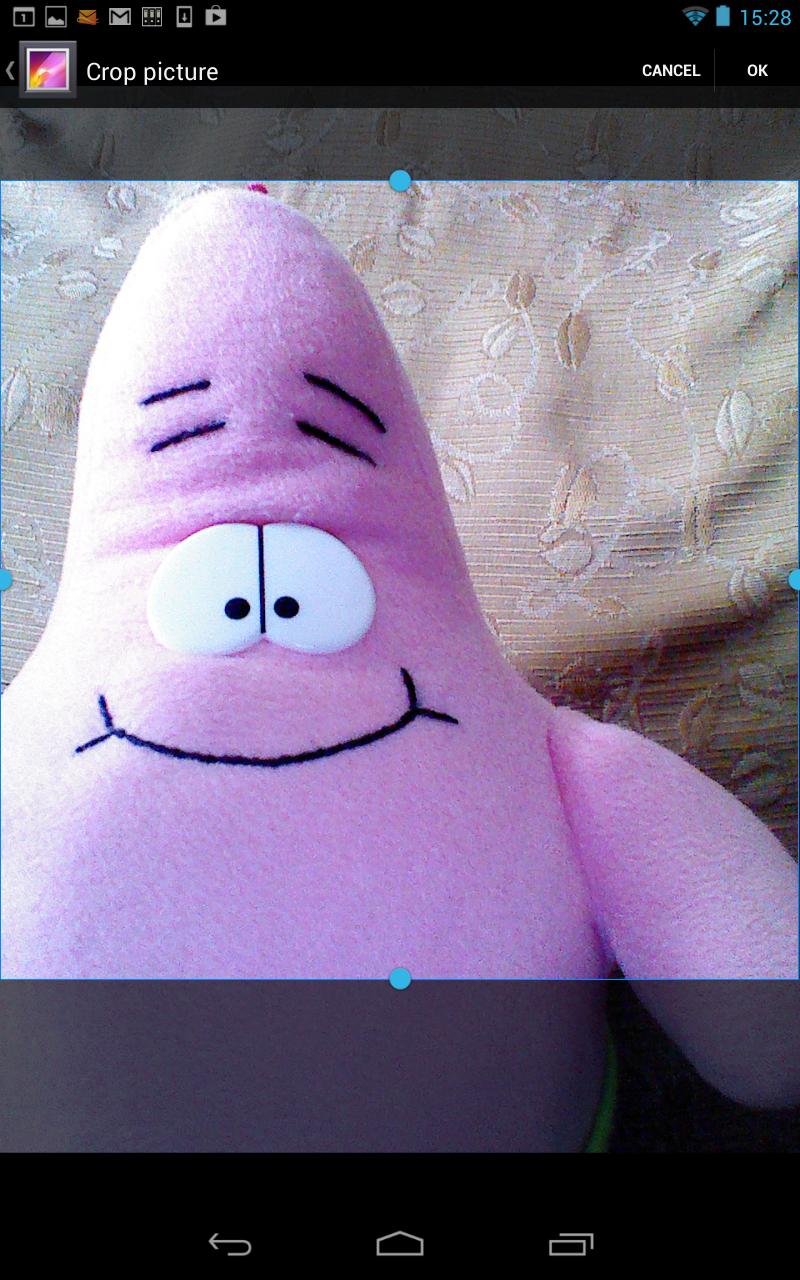
\includegraphics[height=4cm,width=2.8205cm]{imagenes/camaraft1.png}
		\endgroup
	\end{center}

  \begin{block}{}
Una de las caraterísticas básicas que tiene nuestra aplicación es el uso de la cámara. Con ella se pueden tomar las fotos que uno desea para un uso posterior.
  \end{block}

\end{frame}





\begin{frame}
  \frametitle{Drag and Drop}
 

  	\begin{center}
		\begingroup
			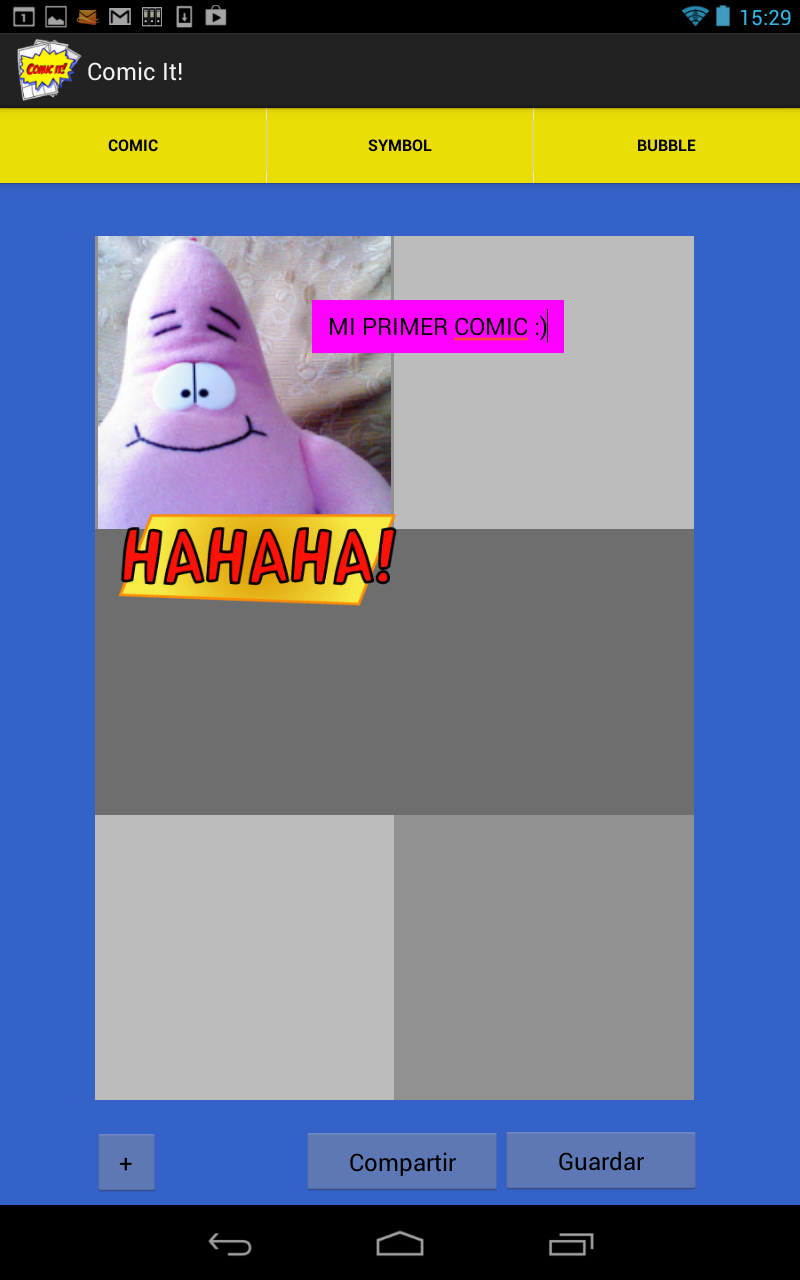
\includegraphics[height=4cm,width=2.8205cm]{imagenes/drag.png}
		\endgroup
	\end{center}

  \begin{block}{}
Una funcionalidad muy divertida: Arrastrar y Soltar. Aquí podrás colocar donde quieras varios textos e íconos predeterminados 
  \end{block}

\end{frame}


\begin{frame}
  \frametitle{Guardar en Galería}
 

  	\begin{center}
		\begingroup
			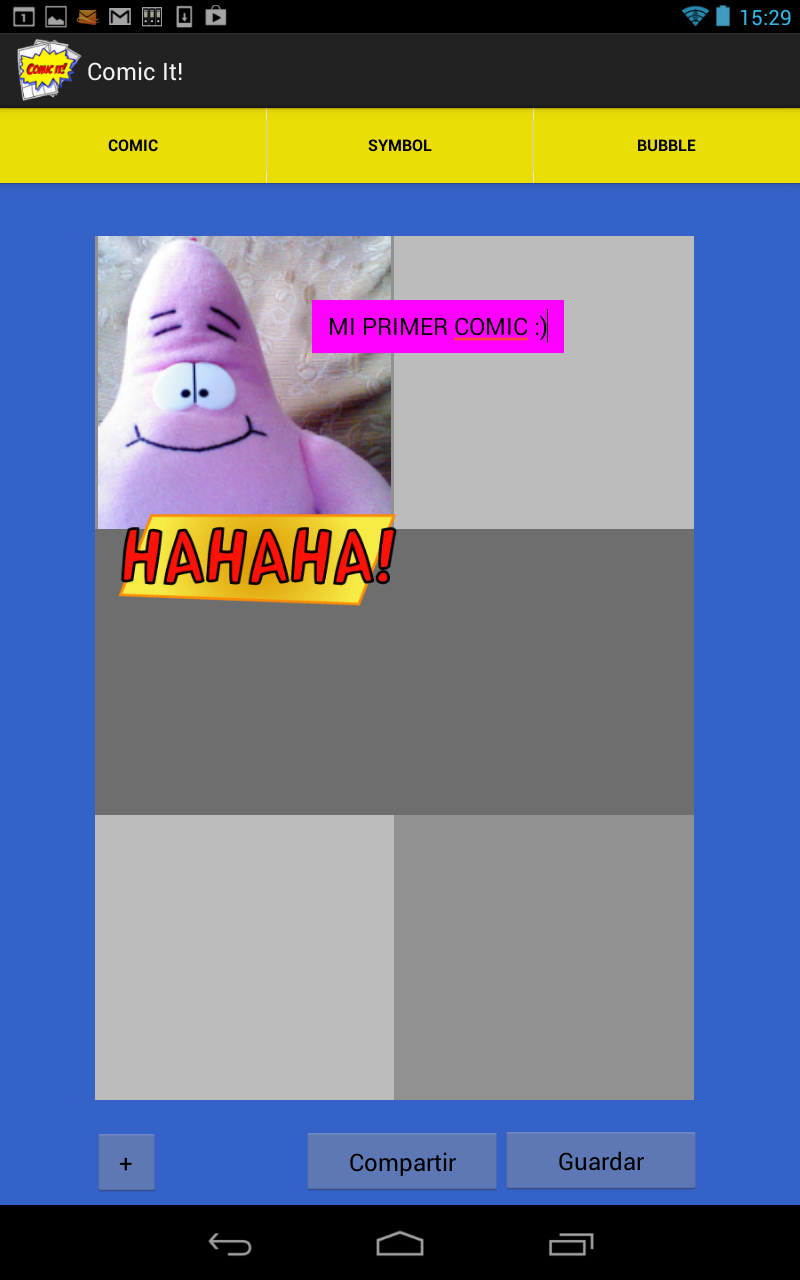
\includegraphics[height=4cm,width=2.8205cm]{imagenes/drag.png}
		\endgroup
	\end{center}

  \begin{block}{}
En la parte inferior derecha se encuentra el botón guardar. Una vez que lo presionas, obtendrás automáticamente tu nuevo Comic en tu galería Android.
  \end{block}

\end{frame}













\end{document}